\documentclass[12pt,a4paper,twocolumn]{article}
\usepackage[margin=15mm,bottom=30mm,footskip=15mm]{geometry}
\usepackage{multicol}
\usepackage{graphicx}
\usepackage{titlesec}
\usepackage{cite}
\usepackage{caption}
\usepackage{subcaption}
\usepackage{hyperref}

\titleformat{\section}{\Large\scshape\centering}{\romannumeral\thesection.}{3mm}{}
\setlength{\columnsep}{6mm}
\setlength{\belowcaptionskip}{-10pt}
\renewcommand{\thesubfigure}{\arabic{subfigure}}
\hypersetup{colorlinks=true}

\begin{document}
    \begin{titlepage}
        \centering

        \vspace*{2cm}
        \begin{figure}[h]
            \centering
            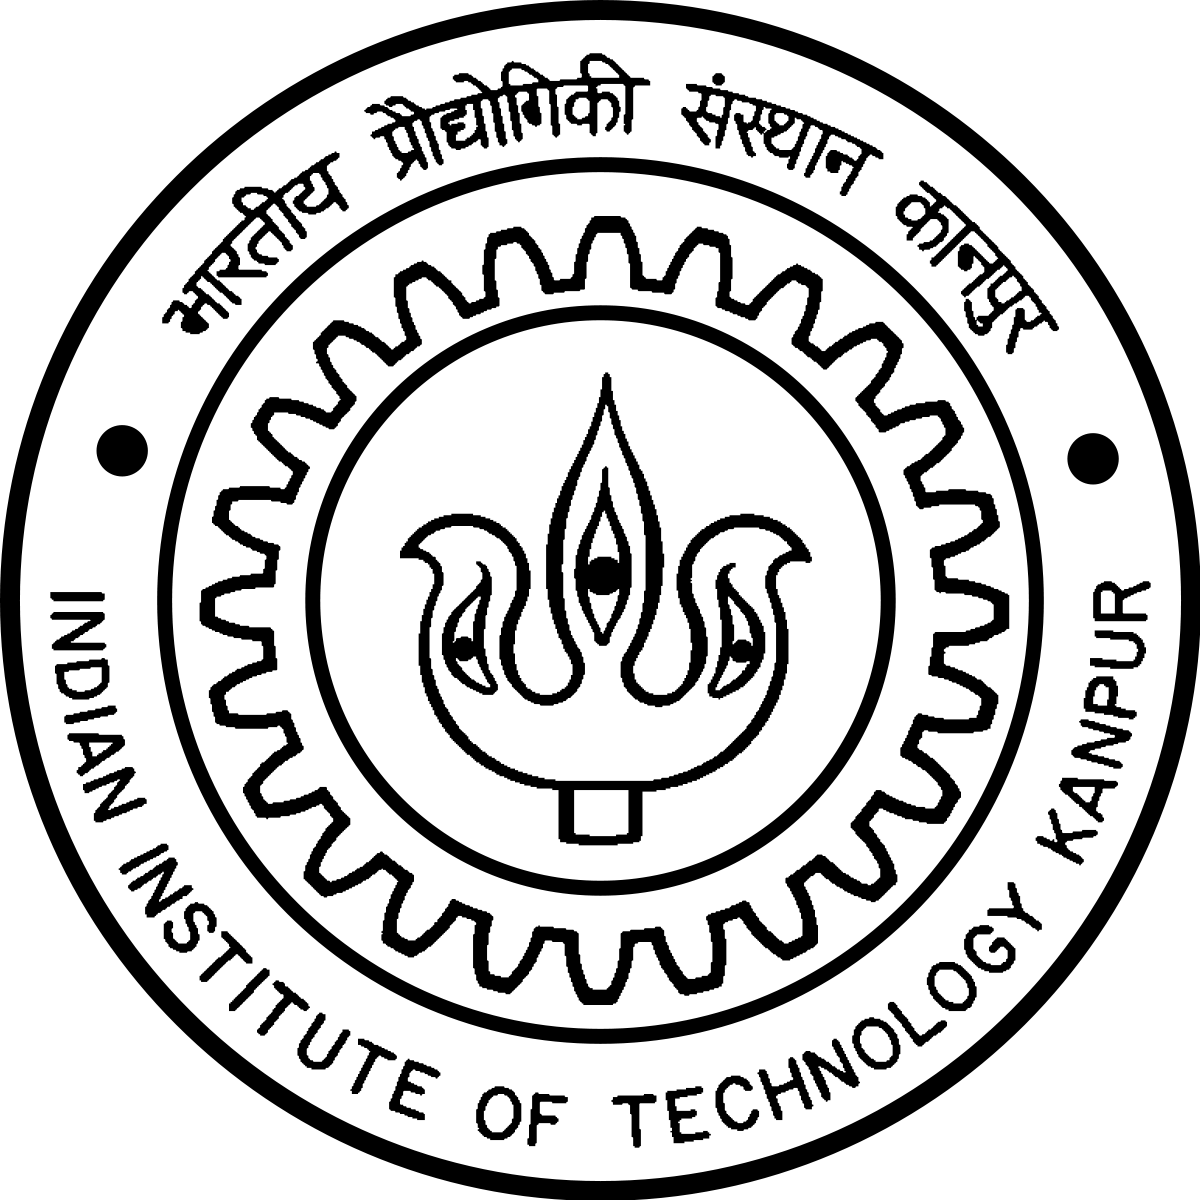
\includegraphics[width=0.3\textwidth]{images/iitk-logo.png}\\[15mm]
        \end{figure}
        \textsc{\LARGE Indian Institute of Technology Kanpur}\\[1cm]
        {\Large CS395A}\\[7mm]

        \hrule
        \vspace{3mm}
        \textbf{\Large Undergraduate Project - 1}\\[5mm]
        \hrule
        \vspace{3mm}

        \begin{multicols}{2}
            \textit{Students:}\\[2mm]
            Harish Rajagopal (160552)\\
            Vishwas Lathi (160808)\\

            \vfill\null\columnbreak

            \textit{Professor:}\\[2mm]
            Vinay Namboodiri\\
            Dept. of Computer Science and Engineering
        \end{multicols}
    \end{titlepage}

    \twocolumn[
        \centering\LARGE Project Report
        \vspace{15mm}
    ]

    \section{Abstract}
        We propose MAD-SRGAN which is multi-agent generalization to SRGAN \cite{srgan}.
        SRGAN, a generative adversarial network \cite{gan} for image super-resolution is capable of generating photo-realistic natural $4\times$ upscaled images.

        SRGAN consists of a single discriminator which tries to discriminate whether generated images are realistic or not, while the generator tries to push the generated image towards the manifold of the natural images.
        MADGAN \cite{madgan} is a generalization of GAN to address the problem of mode collapse, which most of the GAN's and their variants suffer from.
        We propose a modification to vanilla SRGAN by combining MADGAN and SRGAN, namely MAD-SRGAN which consists of multiple generators and further variants also consists of multiple discriminators.

    \section{MAD-SRGAN}
        MAD-SRGAN consists of a $4$ mini-generators each of which which deep residual network \cite{resnet} with skip connections.
        Each residual block consists of two convolution layers with $3\times3$ kernel and $64$ filters followed by batch-normalization \cite{batch-norm} layer and ReLU as the activation function.

        To discriminate whether the generated images lie close to natural images manifold, we have a discriminator network.
        The network uses the DCGAN \cite{dcgan} architecture.
        It consists of $8$ convolution layers with $3\times3$ filter kernels.
        The feature maps obtained from the convolution layers is fed as input to two densely connected layers, which outputs the probability of classification using a sigmoid function.
        The network is trained using high-resolution images which are $4\times$ downscaled and then fed as input to the network while the ground truth remains the upscaled images.

        The input image is divided into $4$ equal and slightly overlapping sections, each corresponding to the top-left, top-right, bottom-left and bottom-right portion of the input image (see fig.~\ref{fig:overlap}).
        Each section is then fed to a mini-generator which tries to generate the corresponding section in the high resolution target image.
        The output of all the generators is concatenated in same fashion as the input image was divided into sections.
        This is then passed as an input to the discriminator which tries to identify whether input image is fake or not.

        @VISHWAS: EXPLAIN MULTI-DISCRIMINATOR SETUP

    \section{Losses}
        The loss function $L$ consists of three parts, namely the content loss $(L_{content})$, adversarial loss $(L_{adv})$ and the overlap loss $(L_{overlap})$.\\
            $$L = L_{content} + \alpha L_{adv} + \beta L_{overlap}$$
        where $\alpha$ and $\beta$ are hyperparameters.

        \begin{figure}
            \centering
            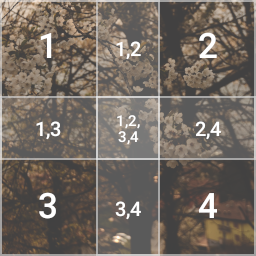
\includegraphics[width=0.3\textwidth]{images/overlap.png}
            \caption{Overlap in outputs}
            \label{fig:overlap}
        \end{figure}

        The content loss is a perceptual loss \cite{perceptual} calculated on feature maps of the VGG19 network \cite{vgg}, similar to the one used by SRGAN.
        The adversarial loss is the adversarial loss for the generators by the discriminator(s).
        The overlap loss is the MSE loss for the overlapping parts of the four generator outputs (see fig.~\ref{fig:overlap}), calculated as follows:
            $$L_{overlap} = \sum_{i=1}^3 \sum_{j=i+1}^4 MSE(i, j)$$
        where $MSE(i, j)$ is the MSE loss for the overlapping parts of images $i$ and $j$.

    \section{Experiments}
        @VISHWAS: DO THIS (MENTION HYPERPARAMETER VALUES, AND CITE Tensorflow \cite{tensorflow} AND MULTI-SCALE SSIM \cite{msssim})

    \section{Results}
        \begin{figure*}
            \centering
            \begin{subfigure}{0.48\textwidth}
                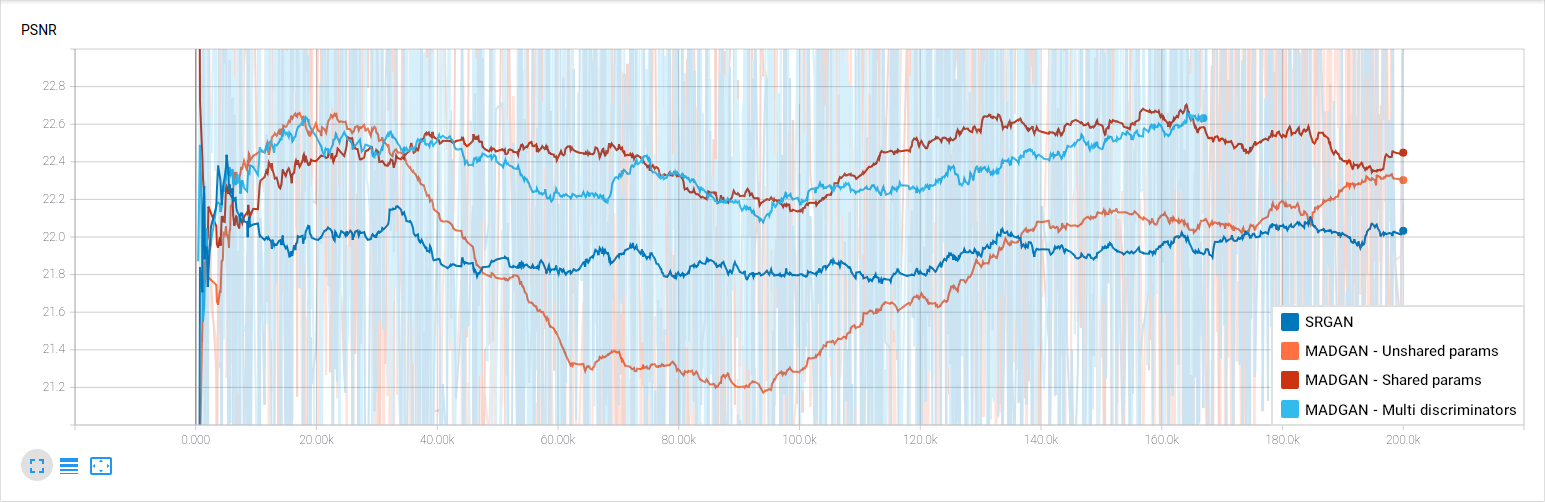
\includegraphics[width=\textwidth]{images/psnr.png}
                \caption{PSNR}\label{psnr-plot}
            \end{subfigure}
            \quad
            \begin{subfigure}{0.48\textwidth}
                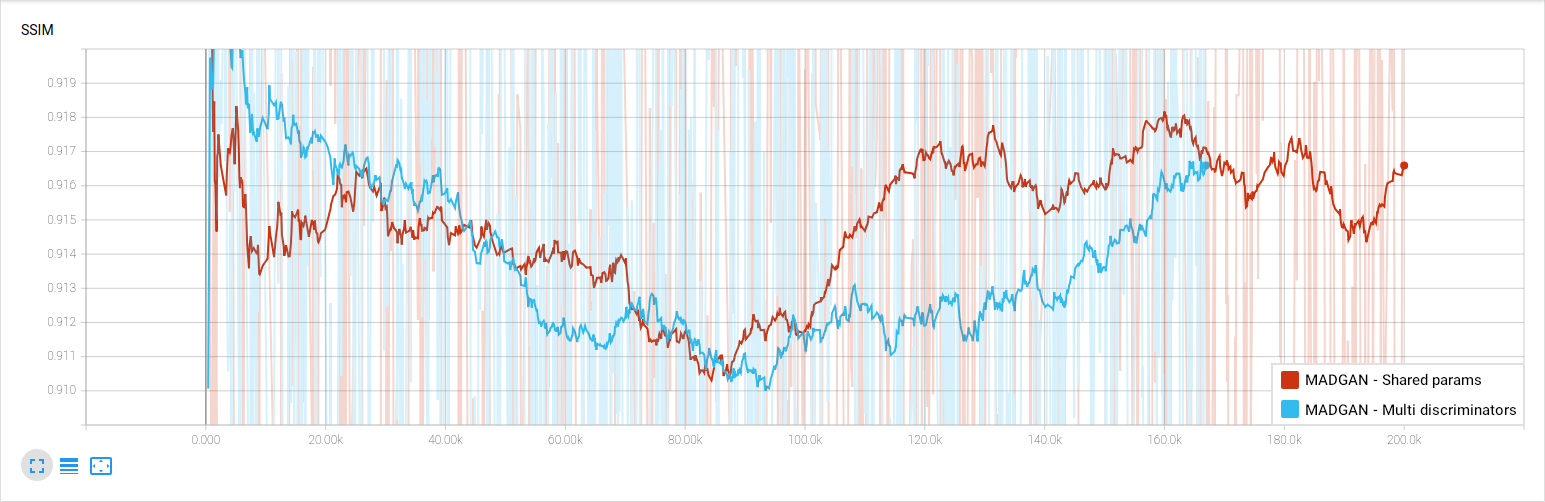
\includegraphics[width=\textwidth]{images/ssim.png}
                \caption{SSIM}\label{ssim-plot}
            \end{subfigure}\\[5mm]
            \begin{subfigure}{0.48\textwidth}
                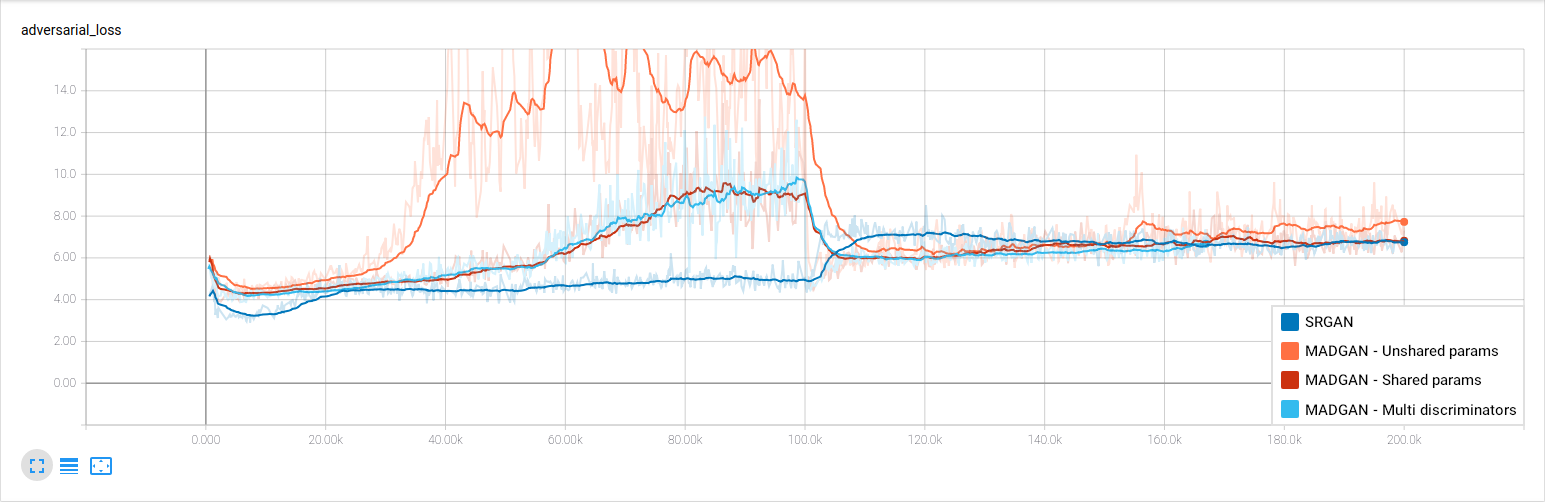
\includegraphics[width=\textwidth]{images/adv-loss.png}
                \caption{Adversarial Loss}\label{adv-loss}
            \end{subfigure}
            \quad
            \begin{subfigure}{0.48\textwidth}
                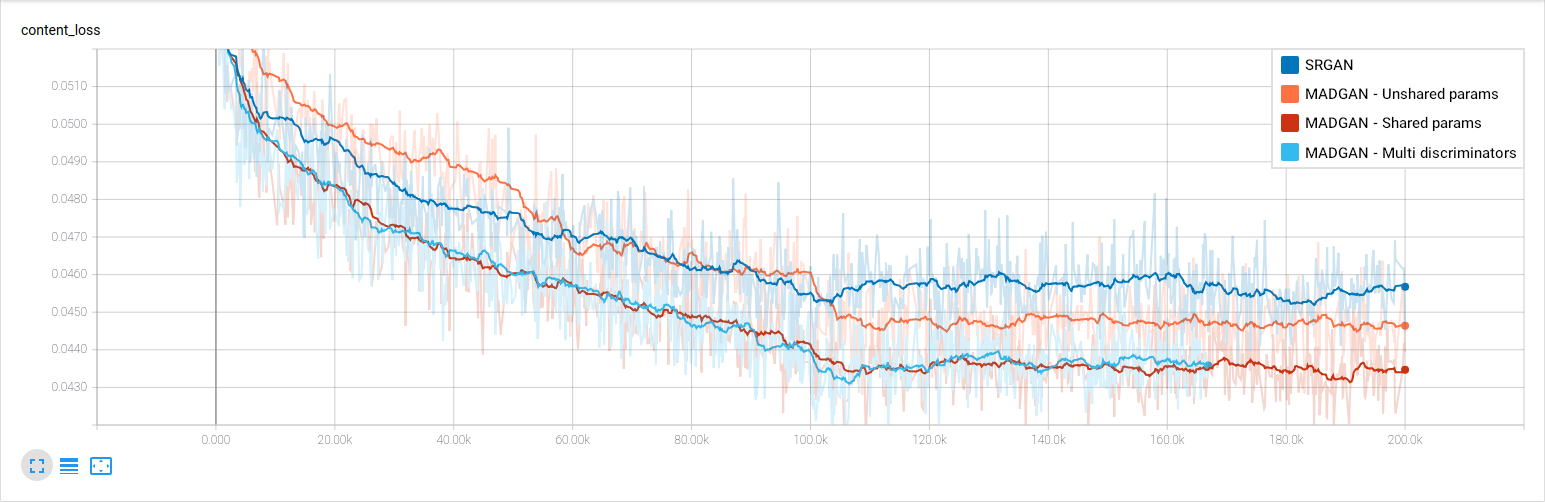
\includegraphics[width=\textwidth]{images/cont-loss.png}
                \caption{Content Loss}\label{cont-loss}
            \end{subfigure}\\[5mm]
            \begin{subfigure}{0.48\textwidth}
                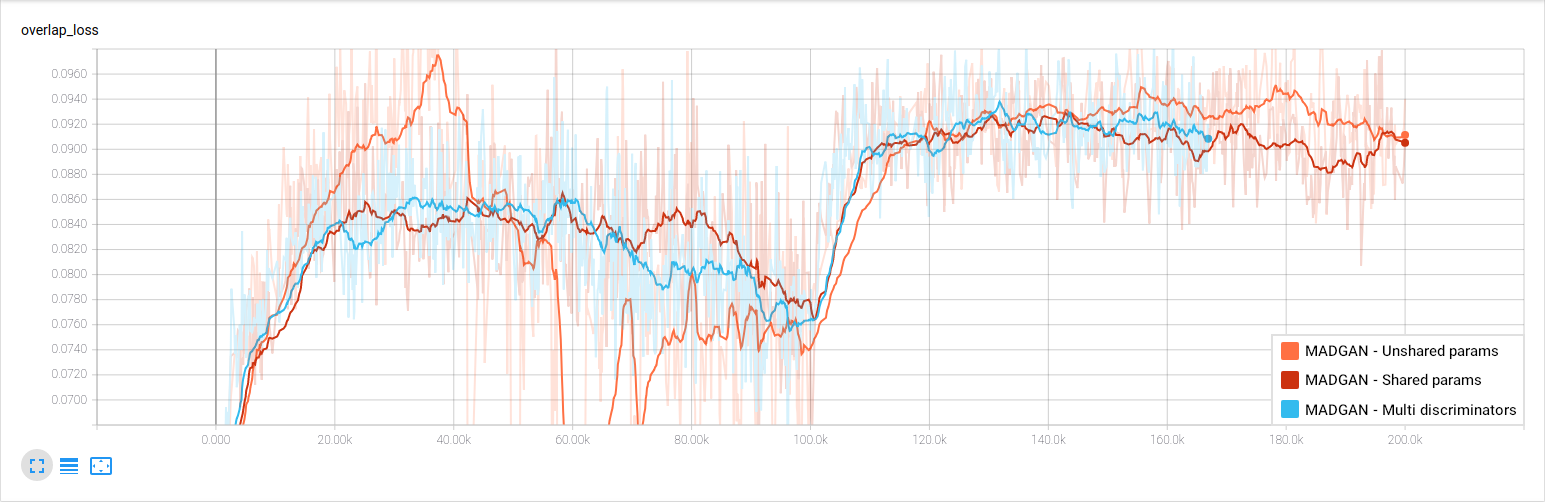
\includegraphics[width=\textwidth]{images/ovrl-loss.png}
                \caption{Overlap Loss}\label{ovrl-loss}
            \end{subfigure}\\[2mm]
            \caption{Results of MAD-SRGAN over SRGAN}
            \label{fig:results}
        \end{figure*}

        Results visualised via Tensorboard \cite{tensorflow} (see fig.~\ref{fig:results}) show that MAD-SRGAN with no sharing of parameters performed poorly as compared to SRGAN.
        Enabling sharing of parameters in the lower layers resulted in a noticeable improvement over keeping parameters separate, and slight improvements over SRGAN.
        We think that this is because sharing results in the lowering of model parameters and thus helps in the stabilization of training those parameters.
        Further, this would help focus the optimizer on fine-tuning the higher layers of the generators as per their requirements and not focus too much on getting the more basic processing required by the lower layers right.

        Addition of multiple discriminators in the form of one discriminator for each generator along with the global discriminator should help to further tune the output of each generator.
        However, we observed that this did not result in a noticeable improvement either in the losses, the metrics (PSNR or SSIM), or even when visually inspecting the output images.

    % Lorem ipsum dolor sit amet\cite{srgan}, consectetur ad ipiscing elit\cite{tensorflow}.
    % Praesent quis bibendum quam.
    % Vivamus finibus non sapien in pellentesque.
    % Mauris auctor a dui id pulvinar.
    % In hac habitasse platea dictumst.
    % Ut a viverra est, eu eleifend massa.
    % Maecenas auctor varius massa, eu interdum quam suscipit sit amet.
    % Pellentesque lobortis imperdiet ex, quis rhoncus nunc cursus ac.
    % Quisque interdum leo in lacinia pellentesque.
    % Praesent interdum rutrum elit, elementum vestibulum lacus mattis ut.
    % Duis consectetur, ex quis efficitur varius, nulla mi imperdiet nisi, et fringilla nisi urna ut lacus.

    % Cras ac quam sodales nisi molestie pretium et sed mi.
    % Vivamus eleifend vitae arcu eu maximus.
    % Vivamus hendrerit eleifend placerat.
    % In nec justo augue.
    % Cras dapibus risus volutpat diam porta, at fermentum purus laoreet.
    % Nam sagittis vitae dui at volutpat.
    % Nunc ullamcorper iaculis justo, vel vestibulum tortor aliquam ac.
    % Vestibulum sed leo purus.
    % Proin at nisl nibh.
    % Phasellus sed scelerisque felis.
    % Etiam ullamcorper quis tellus semper lobortis.

    % Fusce at mauris euismod, faucibus risus sit amet, tempor urna.
    % In hac habitasse platea dictumst.
    % Nulla vel sollicitudin risus.
    % Duis nulla est, condimentum eget eleifend id, mattis et orci.
    % Sed placerat orci sit amet porttitor imperdiet.
    % Morbi in magna in ex molestie porttitor quis a elit.
    % Morbi enim quam, sodales sit amet aliquet elementum, volutpat at sapien.
    % Aliquam in felis non ante vulputate interdum.
    % Duis a cursus nisi.
    % Suspendisse tristique nisl ut tincidunt mollis.
    % Sed tincidunt tortor leo, in bibendum tellus commodo finibus.
    % Phasellus et risus nisl.
    % Etiam mattis neque ligula, ullamcorper vehicula leo tincidunt non.
    % Fusce turpis dui, scelerisque nec vestibulum quis, fringilla tempus libero.
    % Morbi lacus turpis, malesuada at felis ac, tincidunt egestas turpis.

    % In a est quis lectus tempor molestie.
    % In condimentum suscipit faucibus.
    % Ut fermentum erat non lacus lacinia, in porttitor nisi feugiat.
    % Sed sed fermentum purus, sit amet faucibus ex.
    % Etiam finibus metus massa, sed varius quam vestibulum sit amet.
    % Maecenas blandit mi vitae turpis lobortis tempus.
    % Proin sit amet lacus lobortis, lobortis orci a, lobortis erat.
    % Nullam eleifend ante in tempor viverra.
    % Donec efficitur, justo non ultrices molestie, tellus ipsum tempus eros, vel venenatis metus erat non ipsum.
    % Nam massa tellus, accumsan at mauris vel, molestie efficitur nulla.

    \bibliographystyle{ieeetr}
    \bibliography{refer}
\end{document}
